\chapter{АНАЛИЗ ИНСТРУМЕНТОВ И ПОДХОДОВ ПО СОЗДАНИЮ ВЫСОКОНАГРУЖЕННЫХ ВЕБ-ПРИОРЖЕНИЙ} \label{ch2}
	
\section{Виды передачи данных} \label{ch2:title-abbr} 

\textbf{WebSockets} - это тонкий транспортный уровень, построенный поверх стека TCP / IP устройства. Цель состоит в том, чтобы предоставить разработчикам веб-приложений то, что по сути является как можно более близким к исходному уровню связи TCP, при этом добавляя несколько абстракций, чтобы устранить некоторые разногласия, которые в противном случае могли бы существовать в отношении работы Интернета. Они также учитывают тот факт, что в Интернете существуют дополнительные соображения безопасности, которые необходимо учитывать для защиты как пользователей, так и серверов.

\textbf{Long Polling} - – это технология, которая реализует получение информации посредством «Длинных запросов». Механизм производи передачу данных следующим образом. Клиент запрашивает у сервера с помощью обычного http запроса. Сервер получает запрос и отправляет страницу. Данная страница при построении у клиента выполняет специальный скрипт, который отправляет запрос к серверу с указанием флага. Пока не обновится информация на сервере, данный запрос игнорируется. При появлении новой информации или её изменении сервер производит её рассылку. Клиент получает ответ с новой информацией и мгновенно выполняется новый скрипт запроса к серверу, запуская новый процесс ожидания на нём.

\textbf{Server-sent events (SSE)} – эта технология похожа на WebSockets, однако в отличии от неё является односторонним каналом связи. Отправленные события передаются только с сервера на клиент и позволяют клиентам браузера получать поток событий от сервера через соединение HTTP без опроса. Клиент подписывается на «поток» с сервера, и сервер будет отправлять сообщения («поток событий») клиенту, пока сервер или клиент не закроет поток. Сервер сам определяет что и когда отправлять клиенту.

\textbf{Ajax Polling} – технология при которой клиент периодически отправляет серверу запросы XMLHttpRequest / Ajax через определенный интервал для проверки новых данных. Клиент инициирует запросы через небольшие регулярные интервалы (например, 0,5 секунды) Сервер готовит ответ и отправляет его клиенту, как обычные HTTP-запросы. Повторные запросы к серверу тратят ресурсы, так как каждое новое входящее соединение должно быть установлено, HTTP-заголовки должны быть переданы, должен быть выполнен запрос новых данных, а также должен быть сгенерирован и доставлен ответ (обычно без новых данных). Соединение должно быть закрыто и все ресурсы очищены.

\textbf{Forever Frames} – создает скрытый iframe (тэг), который выполняет запрос к конечной точке на сервере, который не завершается. Затем сервер непрерывно отправляет клиенту сценарий, который немедленно выполняется, обеспечивая одностороннее соединение в реальном времени между сервером и клиентом. Соединение от клиента к серверу использует отдельное соединение от сервера к клиентскому соединению, и, как и стандартный HTTP-запрос, новое соединение создается для каждого фрагмента данных, который необходимо отправить.

В табл. \ref{comparisonOfTypesOfDataTransmission} приведены виды транспортировки данных, которые чаще используются.

\begin{table}
	\caption{Сравнение видов передачи данных  \cite{WebSocke87:online,LongPoll65:online,Pollingv75:online}}
	\label{comparisonOfTypesOfDataTransmission}
	\begin{tabularx}{\linewidth}{|X|X|X|X|X|}
		\hline
		& WebSockets & Server-sent events (SSE) &	Long Polling &	Ajax Polling \\
		\hline
		Количество запросов  на опрос сервера &	1 на опрос сервера (установление соединения)	& 1 на опрос сервера (установление соединения)	& 1 на опрос сервера &	1 >= на опрос сервера \\
		\hline
		Количество служебных заголовков вместе с ответом &	1 заголовок в момент подключения клиента к серверу &	1 заголовок в момент подключения клиента к серверу &	1 заголовок за опрос сервера	& 1 заголовок за опрос сервера \\
		\hline
		Служебная информация прикрепляемая в ответе и запросе &	2-10 байт у исходящих, в зависимости от полезной нагрузки &	7-18 байт у исходящие &	~200 байт у запроса и ответа &	~200 байт у запроса и ответа \\
		\hline
	\end{tabularx}
\end{table}

Наилучшим видом передачи данных является WebSockets. Выбор производился с помощью метода Саати (реализация метода Саати Приложение \ref{appendix:methodSaati}).Расчёты можно посмотреть в Приложение \ref{appendix:calculBestTransferDataWay}. Из этого следует, что такой подход предоставляет лучшее решение из представленных вариантов, так как использует меньший объём служебной информации, является двунаправленным, полнодуплексным соединением и для взаимодействия поддерживает одно соединение.
	
\section{Инструменты разработки высоконагруженных приложений} \label{ch2:sec-abbr}
	
\subsection{Введение} \label{ch2:subsec-abbr-introduction} %название по-русски

Разработка любого приложения начинается с разработки архитектуры. Архитектура – это фундамент приложения, который оказывает большое влияние на конечный продукт, в особенности для highload приложения, так как отвечает за успешность и жизнеспособность системы.
	
Спроектировав архитектуру приложения, надо определить его ядро. Ядро обеспечивает связь между веб-клиентами и сервером. Множество языков программирования обладают возможностями для осуществления такого взаимодействия. Кроме того к некоторым из них прилагаются специализированные библиотеки и фреймворки, упрощающие как процесс разработки, так и улучающие  базовый функционал языков. Выбор языка зависит от вида задачи, которую необходимо решить или от требований заказчика. Для высоконагруженных систем условно можно выделить 2 вида:

\begin{itemize}
	\item CPU bound;
	\item I/O bound.
\end{itemize}
	
	
CPU bound (аппаратные ограничения) – задачи связанные с высокой вычислительной сложностью, такие как: специфичные алгоритмы, некоторая математика, задачи кодирования и шифрования и так далее. I/O bound (ограничения на ввод/ вывод) – задачи в которых идут много операции с вводом выводов. Определив вид основной задачи проектируемого приложения определяем ключевые критерии выбора конкретного языка программирования по средством их сравнения (сравнение языков программирования производится точно так же как и в главе «\ref{ch2:title-abbr} \nameref{ch2:title-abbr}»).

Из основных подходов реализации можно выделить:

\begin{itemize}
	\item Разработку приложения средствами самого языка программирования
	\item Разработку приложения совместно с фреймворками и внешних библиотек.
\end{itemize}


На Рис. \ref{fig:ApplicationDevelopmentTools} представлены существующие инструменты для разработки веб-приложений реального времени.

\begin{figure}
	\centering
	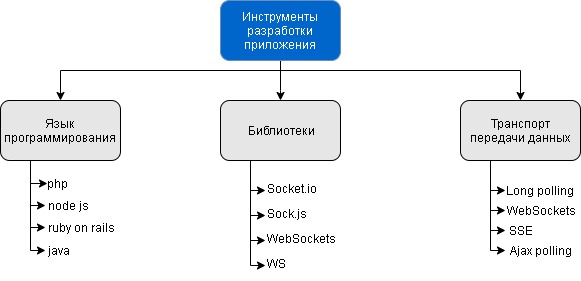
\includegraphics[scale=0.7]{my_folder/images/ApplicationDevelopmentTools}
	\caption{Инструменты разработки приложения}
	\label{fig:ApplicationDevelopmentTools}
\end{figure}
	
\subsection{Языки программирования} \label{ch2:subsec-abbr-programming-languages} %название по-русски









	
%%% ВНИМАНИЕ: для того, чтобы избежать лишнего отступа между текстом  и формулами, пожалуйста, начинайте формулы без пропуска строки в исходном коде как в строках #2 и #3.
Одиночные формулы также, как и отдельные формулы в составе группы, могут быть размещены в несколько строк. Чтобы выставить номер формулы напротив средней строки, используйте окружение \verb|multlined| из пакета \verb|mathtools| следующим образом \cite{Ganter1999}:
\begin{equation} % \tag{S} % tag - вписывает свой текст 
\label{eq:fConcept-order-G}
\begin{multlined}
(A_1,B_1)\leq (A_2,B_2)\; \Leftrightarrow \\  \Leftrightarrow\; A_1\subseteq A_2\; \Leftrightarrow \\ \Leftrightarrow\; B_2\subseteq B_1. 
\end{multlined}
\end{equation}

	
Используя команду \verb|\labelcref{...}| из пакета \verb|cleveref|, допустимо оформить ссылку на несколько формул, например, (\labelcref{eq:UpArrow-G,eq:DownArrow-G,eq:fConcept-order-G}). % пример оформления одиночной формулы в несколько строк

%Пример оформления четырёх иллюстраций в одном текстово-графическом объекте приведён на \firef{fig:spbpu_sc-four-photos}. Это возможно благодаря использованию пакета \verb|subcaption|.

\begin{figure}[ht]
	\adjustbox{minipage=1.3em,valign=t}{\subcaption{}\label{fig:spbpu_sc-a}}%
	\begin{subfigure}[t]{\dimexpr.5\linewidth-1.3em\relax}
		\centering
		
\includegraphics[width=.95\linewidth,valign=t]{my_folder/images/spbpu_sc_system}
	\end{subfigure}
\hfill %выровнять по ширине
	\adjustbox{minipage=1.3em,valign=t}{\subcaption{}\label{fig:spbpu_sc-b}}%
	\begin{subfigure}[t]{\dimexpr.5\linewidth-1.3em\relax}
		\centering
		
\includegraphics[width=.95\linewidth,valign=t]{my_folder/images/spbpu_sc_refr}
	\end{subfigure}
\\[20pt]
	\adjustbox{minipage=1.3em,valign=t}{\subcaption{}\label{fig:spbpu_sc-c}}%
\begin{subfigure}[t]{\dimexpr.5\linewidth-1.3em\relax}
	\centering
	
\includegraphics[width=.95\linewidth,valign=t]{my_folder/images/spbpu_sc_hall}
\end{subfigure}%
\hfill %выровнять по ширине
\adjustbox{minipage=1.3em,valign=t}{\subcaption{}\label{fig:spbpu_sc-d}}%
\begin{subfigure}[t]{\dimexpr.5\linewidth-1.3em\relax}
	\centering
	
\includegraphics[width=.95\linewidth,valign=t]{my_folder/images/spbpu_sc_box}
\end{subfigure}
\captionsetup{justification=centering} %центрировать
\caption{Фотографии суперкомпьютерного центра СПбПУ \cite{spbpu-gallery}: {\itshape a} --- система хранения данных и узлы NUMA-вычислителя; {\itshape b} --- холодильные машины на крыше научно-исследовательского корпуса; {\itshape c} --- машинный зал; {\itshape d} --- элементы вычислительных устройств} 
\label{fig:spbpu_sc-four-photos}
\end{figure}

Далее можно ссылаться на составные части данного рисунка как на самостоятельные объекты: \firef{fig:spbpu_sc-a}, \firef{fig:spbpu_sc-b}, \firef{fig:spbpu_sc-c}, \firef{fig:spbpu_sc-d} или на три из четырёх изображений одновременно: рис.\labelcref{fig:spbpu_sc-a,fig:spbpu_sc-b,fig:spbpu_sc-c}. % пример подключения 4х иллюстраций в одном рисунке

%На \firef{fig:spbpu_whitehall-three-photos} приведены три картинки под~общим номером и~названием, но с раздельной нумерацией подрисунков посредством пакета \verb|subcaption|.
%
\begin{figure}[!htbp]
	\adjustbox{minipage=1.3em,valign=t}{\subcaption{}\label{fig:spbpu_whitehall-a}}%
	\begin{subfigure}[t]{\dimexpr.3\linewidth-1.3em\relax}
		\centering
		
\includegraphics[width=.95\linewidth,valign=t]{my_folder/images//spbpu_whitehall}
	\end{subfigure}
	\hfill %выровнять
	\adjustbox{minipage=1.3em,valign=t}{\subcaption{}\label{fig:spbpu_whitehall-b}}%
	\begin{subfigure}[t]{\dimexpr.3\linewidth-1.3em\relax}
		\centering
		
\includegraphics[width=.95\linewidth,valign=t]{my_folder/images//spbpu_whitehall_ligh}
	\end{subfigure}
	\hfill %выровнять
		\adjustbox{minipage=1.3em,valign=t}{\subcaption{}\label{fig:spbpu_whitehall-c}}%
	\begin{subfigure}[t]{\dimexpr.3\linewidth-1.3em\relax}
		\centering
		
\includegraphics[width=.95\linewidth,valign=t]{my_folder/images//spbpu_whitehall_sculpture}
	\end{subfigure}%
\captionsetup{justification=centering} %центрировать
	\caption{Фотографии Белого зала СПбПУ \cite{spbpu-gallery}, в том числе: {\itshape a} --- со стороны зрителей; {\itshape b} --- со стороны сцены; {\itshape c} --- барельеф}\label{fig:spbpu_whitehall-three-photos}  
\end{figure}

Далее можно ссылаться на три отдельных рисунка: \firef{fig:spbpu_whitehall-a}, \firef{fig:spbpu_whitehall-b} и \firef{fig:spbpu_whitehall-c}. % пример подключения 3х иллюстрации в одном рисунке
%
%На \firef{fig:spbpu_main_bld-two-photos} приведены две картинки под~общим номером и~названием.


\begin{figure}[!htbp]
	\adjustbox{minipage=1.3em,valign=t}{\subcaption{}\label{fig:spbpu_main_bld_entrance_autumn}}%
	\begin{subfigure}[t]{\dimexpr.5\linewidth-1.3em\relax} %разрешили выделить 0,5 стр в ширину на рисунок
		
\includegraphics[height=0.20\textheight,valign=t]{my_folder/images//spbpu_main_bld_entrance_autumn} %высоту рисунка выставили как 0,3 от высоты наборного поля
	\end{subfigure}
%	\hfill %выровнять по ширине
	\adjustbox{minipage=1.3em,valign=t}{\subcaption{}\label{fig:spbpu_main_bld_whitehall}}%
	\begin{subfigure}[t]{\dimexpr.5\linewidth-1.3em\relax}%разрешили выделить 0,5 стр в ширину на рисунок
		
\includegraphics[height=0.20\textheight,valign=t]{my_folder/images//spbpu_main_bld_whitehall}%высоту рисунка выставили как 0,3 от высоты наборного поля
	\end{subfigure}
\captionsetup{justification=centering} %центрировать
	\caption{Вид на главное здание СПбПУ \cite{spbpu-gallery}, включая: {\itshape a} --- вход со стороны парка осенью; {\itshape b}~--- окна Белого зала}\label{fig:spbpu_main_bld-two-photos} 
\end{figure}

На \firef{fig:spbpu_main_bld_entrance_autumn} изображен вход со стороны парка СПбПУ осенью, а на \firef{fig:spbpu_main_bld_whitehall}~--- окна Белого зала. % пример подключения 2х иллюстраций в одном рисунке

%Приведём пример табличного представления данных с записью продолжения на следующей странице на \taref{tab:long}.

%%% отладка longtable
%% 1) для контроля выхода таблицы за границы полей выставляем showframe в \geometry{}, см настройки
%% 2) используем \\* для запрета переноса определенной строки или средства из:
%% https://tex.stackexchange.com/q/344270/44348
%% 3) в крайнем случае для принудительного переноса таблицы на новую страницу используем \pagebreak после \\
\noindent % for correct centering
\begingroup
\centering
\small %выставляем шрифт в 12bp
\begin{longtable}[c]{|l|l|l|l|l|l|}
	\caption{Пример задания данных из \cite{Peskov2004} (с повтором для переноса таблицы на новую страницу)}%
	\label{tab:long}% label всегда желательно идти после caption
	\\
	\hline
	$G$&$m_1$&$m_2$&$m_3$&$m_4$&$K$\\ \hline
	1&2&3&4&5&6\\ \hline
	\endfirsthead%
	\captionsetup{format=tablenocaption,labelformat=continued} % до caption!
	\caption[]{}\\ % печать слов о продолжении таблицы
	\hline
	1&2&3&4&5&6\\ \hline
	\endhead
	\hline
	\endfoot
	\hline
	\endlastfoot
	$g_1$&0&1&1&0&1\\ \hline
	$g_2$&1&2&0&1&1\\ \hline
	$g_3$&0&1&0&1&1\\ \hline
	$g_4$&1&2&1&0&2\\ \hline
	$g_5$&1&1&0&1&2\\ \hline
	$g_6$&1&1&1&2&2\\ \hline
%
	$g_1$&0&1&1&0&1\\ \hline 
	$g_2$&1&2&0&1&1\\ \hline
	$g_3$&0&1&0&1&1\\ \hline
	$g_4$&1&2&1&0&2\\ \hline \noalign{\penalty-5000} % способствуем переносу на следующую стр
	$g_5$&1&1&0&1&2\\ \hline 
	$g_6$&1&1&1&2&2\\ \hline
%
	$g_1$&0&1&1&0&1\\ \hline 
	$g_2$&1&2&0&1&1\\ \hline
	$g_3$&0&1&0&1&1\\ \hline
	$g_4$&1&2&1&0&2\\ \hline
	$g_5$&1&1&0&1&2\\ \hline
	$g_6$&1&1&1&2&2\\ \hline
%		
	$g_1$&0&1&1&0&1\\ \hline 
	$g_2$&1&2&0&1&1\\ \hline
	$g_3$&0&1&0&1&1\\ \hline
	$g_4$&1&2&1&0&2\\ \hline
	$g_5$&1&1&0&1&2\\ \hline
	$g_6$&1&1&1&2&2\\ \hline
%
	$g_1$&0&1&1&0&1\\ \hline 
	$g_2$&1&2&0&1&1\\ \hline
	$g_3$&0&1&0&1&1\\ \hline
	$g_4$&1&2&1&0&2\\ \hline
	$g_5$&1&1&0&1&2\\ \hline
	$g_6$&1&1&1&2&2\\ \hline
%
	$g_1$&0&1&1&0&1\\ \hline 
	$g_2$&1&2&0&1&1\\ \hline
	$g_3$&0&1&0&1&1\\ \hline
	$g_4$&1&2&1&0&2\\ \hline
	$g_5$&1&1&0&1&2\\ \hline
	$g_6$&1&1&1&2&2\\ \hline
%
	$g_1$&0&1&1&0&1\\ \hline 
	$g_2$&1&2&0&1&1\\ \hline
	$g_3$&0&1&0&1&1\\ \hline
	$g_4$&1&2&1&0&2\\ \hline
	$g_5$&1&1&0&1&2\\ \hline
	$g_6$&1&1&1&2&2\\ \hline
\end{longtable}
\normalsize% возвращаем шрифт к нормальному
\endgroup % пример подключения таблицы на несколько страциц








Выбор правильного языка программирования имеет решающее значение в разработке приложения. Проведём исследование языков программирования, подходящих для серверной веб-разработки, таких как Python, Node.js, Java, PHP. Языки сравниваются по общей популярности, поддержке облачных провайдеров, производительности и доступным интеграциям.

\textbf{Python} – это интерпретируемый объектно-ориентированный язык программирования высокого уровня с динамической семантикой. Его встроенные структуры данных высокого уровня в сочетании с динамической типизацией и динамическим связыванием делают его очень привлекательным для быстрой разработки приложений, а также для использования в качестве скриптового или связующего языка для соединения существующих компонентов. Python поддерживает модули и пакеты, что способствует модульности программы и повторному использованию кода. Интерпретатор Python и обширная стандартная библиотека доступны для всех основных платформ.

\textbf{Node.js} – это среда, которая позволяет использовать JavaScript как для backend, так и для frontend разработки, а также для решения проблем совместимости. Его также можно определить как язык сценариев на стороне сервера. Он хорош для обработки проектов с множеством одновременных подключений или приложений с высокоскоростным и интенсивным вводом / выводом (I/O), а также приложений, таких как платформы повышенной производительности (например, системы управления контентом), торговые площадки P2P и платформы электронной коммерции.

\textbf{Java} – это объектно-ориентированный и параллельный язык программирования общего назначения, разработанный Sun Microsystems в 1995 году. Он использует механизм под названием JVM (виртуальная машина Java), который обеспечивает среду выполнения для запуска кода Java и его приложений. Он переводит байт-код Java в язык, который может интерпретироваться машинами. JVM является частью JRE (Java Runtime Environment).

\textbf{PHP} – это язык программирования, созданный для создания веб-приложений, построенный на языке программирования C и использующий уникальные HTML-подобные теги для содержания своего кода. Язык программирования PHP в основном используется на стороне сервера, что означает, что он работает на программном обеспечении вашего веб-сервера, которое обычно будет обслуживать HTML ваших посетителей.


\begin{table}
	\caption{Сравнение языков программирования  \cite{PHPvsPyt48:online,NodejsVs38:online} Приложение \cite{appendix:comparationPL}}
	\label{comparisonOfProgrammingLanguage}
	\begin{tabularx}{\linewidth}{|X|X|X|X|X|}
		\hline
		& Python & Node Js & Java & PHP \\
		\hline
		Наличие библиотек & Обладает исключительно хорошо развитой библиотечной поддержкой практически для всех типов приложений & Обладает исключительно хорошо развитой библиотечной поддержкой практически для всех типов приложений & Hibernate, Swing, SWT (Standard Widget Toolkit) & Packagist (репозиторий пакетов PHP) является сильной основой, поддерживающей PHP \\
		\hline
		Доступ к базам данных & Не сильная интеграция базы данных & Он обеспечивает доступ к более чем 20 различным базам данных & Он обеспечивает доступ к более чем 20 различным базам данных & Он обеспечивает доступ к более чем 20 различным базам данных \\
		\hline
		Скорость работы & 4/5 & 5/5 & 5/5 & 4/5 \\
		\hline
		Наличие фреймворков & Django, Flask, Pylons, Pyramid & Express.js, Meteor.js, Koa.js & Java Server Faces (JSF), Stuts2, Spring & Codeigniter, Zend, Laravel, Symfony \\
		\hline
	\end{tabularx}
\end{table}

Наилучшим языком программирования, согласно представленным критериям и по расчётам  метода Саати – является Java (Приложение \ref{appendix:methodSaati}). Из этого следует, что такой подход предоставляет лучшее решение из представленных вариантов, однако в разработке для сервера будет использоваться Node js (согласно требованиям заказчика).

\subsection{Библиотеки}

Чтобы обеспечить двустороннюю связь клиента с сервером выделим решения, считающиеся популярными, для работы с web sockets и Node.js.

Socket.io – это библиотека позволяет установить двунаправленную связь между клиентом и сервером. Для корректной работы библиотеки, ей необходимо установить как на клиентской стороне, так и на серверной Node js. API у компонент (клиентская, серверная) – идентичен и управляет событиями. Socket.IO напоминает WebSockets. WebSockets также является браузерной реализацией, позволяющей осуществлять двунаправленную связь, однако Socket.IO не использует это в качестве стандарта. Во-первых, Socket.IO создает соединение с длинным опросом, используя xhr-опрос. Затем, как только это установлено, он обновляется до наилучшего способа подключения. В большинстве случаев это приведет к соединению WebSocket. Хотя Socket.IO может использоваться в качестве оболочки для WebSocket так как предоставляет больший функционал, включая широковещательную передачу на несколько сокетов, асинхронный ввод-вывод и хранение данных.

Sock.js - то JavaScript-библиотека браузера, которая предоставляет объект, подобный WebSocket. SockJS предоставляет вам согласованный кросс-браузерный API Javascript, который создает полнодуплексный междоменный канал связи с низкой задержкой между браузером и веб-сервером.

Произведём сравнение WebSocket \cite{WebSocke16:online} с популярными библиотеками \cite{Introduc57:online,SockJS·G77:online}, работающими на этом протоколе, однако предлагающими больший функционал. Для сравнения были разработаны клиенты и серверы (Приложения \ref{appendix:serverSideBySocketIO}, \ref{appendix:serverSideBySockJS}), используя express.js (фреймворк для создания сервера Node.JS).



\begin{figure}
	\centering
	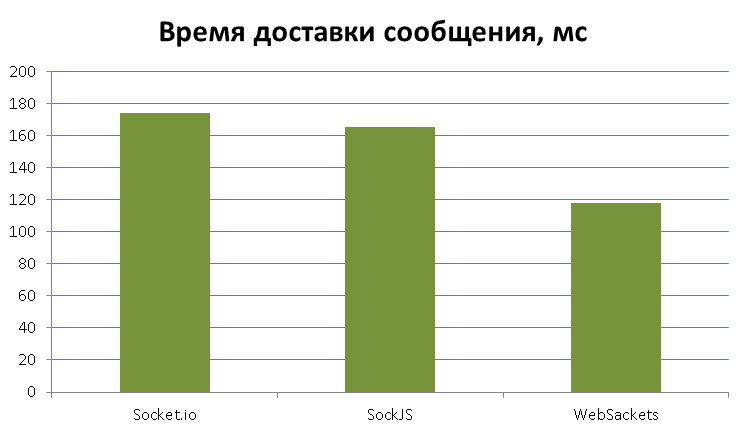
\includegraphics[scale=0.7]{my_folder/images/speedMessageDeliver}
	\caption{Сравнение времени опроса}
	\label{fig:speedMessageDeliver}
\end{figure}

\subsection{Мониторинг}
\label{Moninoring}

%\FloatBarrier % заставить рисунки и другие подвижные (float) элементы остановиться
Так как веб-серверы обрабатывают запросы пользователей на контент, то это непосредственно отражается на производительности и заметное влияние на взаимодействие с пользователя. Если веб-серверы работают медленно, пользователи откажутся от его услуг. Поэтому Application Performance Monitoring (APM) необходим для проекта. Он предупредит вас о любых ошибках или сбоях, которые могут привести к простою и о возможных сбоях.

Одним из основных преимуществ мониторинга – автоматизация. Сайты высокой ежедневной проходимостью часто оптимизируют пропускную способность балансировкой нагрузки, когда запросы делегируются на несколько веб-серверов. Отдельная служба балансировки нагрузки принимает входящие запросы, проверяет доступность веб-серверов, расположенных за ней, и передает запрос на доступный сервер. Для этого балансировщик нагрузки должен знать текущую нагрузку каждого веб-сервера и его доступность для обработки новых запросов.

Наконец, мониторинг помогает отслеживать популярность и рост веб-сайтов и веб-приложений. Метрики трафика и подключений позволяют получить непосредственное представление об активности сайта, в том числе о количестве активных пользователей и продолжительности каждого сеанса. Эти данные могут помочь вам разработать планы по масштабированию вашего веб-сайта, оптимизации вашего приложения или развертыванию других служб для поддержки возросшего спроса.

\textbf{New Relic} – является одним из самых популярных инструментов в среде APM. Он предоставляет информацию о многих типах программных и аппаратных компонентов или о взаимодействии с пользователем и поддерживает множество технологий, либо через своих собственных агентов, либо через внешние плагины. Одной из лучших функций является подробный мониторинг транзакций, обеспечивающий отслеживание между приложениями и отслеживание производительности операторов SQL. \cite{NewRelic78:online}

Преимущества:
\begin{itemize}
	\item Дружественный пользовательский интерфейс;
	\item Очень хорошо в нахождении корреляции данных;
	\item Включает отслеживание транзакций и процессов;
	\item Хороший форум сообщества и поддержка.
\end{itemize}

Недостатки:
\begin{itemize}
	\item Предоставляется только по SaaS (нет локальной версии);
	\item Хранение данных зависит от уровня подписки, но в лучшем случае сохраняет все данные в течение 8 дней (после сохраняет только усреднённые данные);
	\item Ценообразование. Стоимость подписки начинается примерно с 60 долларов США за месяц и увеличивается в зависимости от многих аспектов (уровня подписки, компонентов мониторинга, количества серверов и т. д.). С другой стороны, он имеет бесплатную версию Lite, но она сильно урезана и имеет только 2 часа хранения ограниченного количества данных (строго определённых).
\end{itemize}

\textbf{CloudWatch} – это инструмент мониторинга и управления Amazon Web Service (AWS). Он предоставляет данные о производительности компонентов AWS и приложений, работающих в инфраструктуре Amazon. CloudWatch имеет базовый мониторинг, который является бесплатным для пользователей AWS, а так же подобрав тарифный план его можно улучшить. Предоставляя такие функции, как более подробный мониторинг, пользовательские метрики и многое другое. Однако пользовательский интерфейс может быть немного сложным для людей, не имеющих опыта работы с подобными инструментами.\cite{AmazonCl81:online}

Преимущества:
\begin{itemize}
	\item Бесплатная версия (для пользователей AWS) предлагает достаточно ресурсов для базового мониторинга приложения;
	\item Настраиваемые панели для отображения метрик и графиков;
	\item Гибкие низкие цены.
\end{itemize}

Недостатки:
\begin{itemize}
	\item Он может использоваться только для компонентов AWS и, следовательно, для приложений, работающих только на серверах Amazon. Есть несколько скриптов, созданных сторонними разработчиками, для получения метрик для серверов не-AWS, но они не являются «официальным»;
	\item Пользовательский интерфейс не очень удобен для анализа данных, что затрудняет выполнение корреляции данных;
	\item Нет отслеживания транзакций;
	\item По умолчанию нет метрик использования памяти. Пользовательский показатель должен быть настроен для мониторинга этого основного индикатора.
\end{itemize}

\textbf{Dynatrace APM} – предлагает мониторинг производительности и управление приложениями как в модели SaaS, так и на локальном сервере. Он поддерживает несколько технологий, имеет глубокую трассировку транзакций, мониторинг взаимодействия с пользователем (синтетический мониторинг и мониторинг реального пользователя) и мониторинг сети. Так присутствует функция, которая автоматически обнаруживает все компоненты сервера и быстро запускает отчетные данные на разных уровнях после его установки. Даже время загрузки страницы сообщается путем внедрения JavaScript в ваше веб-приложение.\cite{Applicat35:online}

Преимущества:
\begin{itemize}
	\item Простота установки и настройки;
	\item Бесплатная версия позволяет контролировать до 5 серверов в течение неограниченного времени, без ограничений функциональности или срока хранения данных. Там количество посещений ограничено 100к;
	\item Обнаруживает топологию приложений, развертывания и изменения среды в режиме реального времени;
	\item Отлично подходит для отслеживания транзакций и процессов.
\end{itemize}

Недостатки: 
\begin{itemize}
	\item Пользовательский интерфейс немного сложен, особенно для пользователей, не имеющих опыта работы с подобными инструментами;
	\item Ценообразование. Несмотря на то, что бесплатная версия действительно хороша для небольших инфраструктур (5 серверов или меньше), платные опции имеют цены, аналогичные New Relic.
\end{itemize}


\textbf{AppDynamics} – несколько лет назад этот инструмент был основным современным программным обеспечением для мониторинга APM. Рассматривая некоторые функции AppDynamics (например, главный экран с картой служб, используемых с их нагрузкой на вызов и индексом работоспособности, или мониторами взаимодействия с пользователем), создается впечатление, что приоритетами мониторинга инструментов являются крупные предприятия с большой инфраструктурой.\cite{Theworld87:online}

Преимущества:
\begin{itemize}
	\item Дружественный пользовательский интерфейс с настраиваемыми инструментальными панелями;
	\item Хороший мониторинг ресурсов сервера;
	\item Включает транзакции и отслеживание процессов;
	\item Использует алгоритмы машинного обучения, чтобы установить базовые значения для установки оповещения.
\end{itemize}

Недостатки:
\begin{itemize}
	\item Некоторые функции инструмента основаны на Flash, и вы не можете использовать их, не включив его в браузере;
	\item Ценообразование. AppDynamics нет цен, опубликованных на веб-странице, вам придется связаться с отделом продаж, чтобы получить индивидуальный план и стоимость, основанные на ваших потребностях.
\end{itemize}


\textbf{CA Technologies APM} – одной из основных характеристик инструмента CA APM является то, что это гибкое и настраиваемое программное обеспечение: компания предлагает службу поддержки, которая позволяет настраивать особый мониторинг и оповещения для получения более точных и полезных данных для каждого специфическая для компании ситуация. 

CA APM имеет настраиваемые панели мониторинга, многоперспективные представления о работе конечных пользователей, автоматические трассировки транзакций и множество показателей ресурсов инфраструктуры.\cite{Applicat77:online}

Преимущества:
\begin{itemize}
	\item Универсальный инструмент, так как компания CA готова адаптировать инструмент для нужд клиента;
	\item Team Center предоставляет настраиваемую панель инструментов для быстрой навигации по деталям, чтобы разобраться в проблемах;
	\item Включает отслеживание транзакций и процессов;
	\item Хорошая поддержка и форум сообщества.
\end{itemize}

Недостатки:
\begin{itemize}
	\item Это может потребовать довольно большой кривой обучения, особенно для людей, не имеющих опыта работы с такими инструментами;
	\item Цены могут быть немного высокими для небольших инфраструктур.
\end{itemize}



\begin{table}
	\caption{Сравнение APM}
	\label{comparisonOfAPM}
	\begin{tabularx}{\linewidth}{|p{1.8cm}|X|X|X|X|X|}
		\hline
	& User Interface &	SaaS/ Local server	& Transaction trecking	& Data correlation & Support services\\
		\hline
		New Relic &	Простой и понятный интерфейс &	SaaS	& Подробный мониторинг транзакций	& Хорошо реализован	& Имеется \\
		\hline
		Cloud Watch &	Требует определённые навыки работы в данной сфере & 	SaaS и локальный сервер (только для AWS) & 	Отсутствует	& Имеется, слабая реализация	& Имеется, но только для клиентов AWS \\
		\hline
		Dynatrace APM	& В начале кажется сложным, но к нему быстро привыкнуть	& SaaS и локальный сервер & 
		Отличное (подробное) отслеживание проходящих транзакций и процессов	& Хорошо реализован	& Имеется, но уровень помощи зависит от подписки \\
		\hline
		App Dynamics	& Простой и понятный интерфейс, только используется Flash	& SaaS и локальный сервер	& Подробный мониторинг транзакций	& Имеется	& Имеется \\
		\hline
		CA APM	& Простой и понятный интерфейс	& SaaS и локальный сервер	& Подробный мониторинг транзакций	& Хорошо реализован	& Имеется \\
		\hline		
	\end{tabularx}
\end{table}

\newpage

%%%%%%%%%%%%%%%%%%%%%%%%%%%%%%%%%%%%%%%%%%%%
%
%    Не забыть поменять ссылку на Приложение 
%
%%%%%%%%%%%%%%%%%%%%%%%%%%%%%%%%%%%%%%%%%%%%
Наилучшей системой мониторинга, согласно представленным критериям и по расчётам  метода Саати – является Dynatrace APM (Приложение \ref{appendix:choosingMonitoringSys}). Из этого следует, что такой подход предоставляет лучшее решение мониторинга из выше представленных.


\subsection{Веб-хостинг}
\label{web_hosts}

\subsubsection{Виды хостингов}
\label{typeOfHosts}

Выбирать хостинг, на котором будет размещаться высокопроизводительное веб-приложение – это ещё один важный пункт. Если все сделано правильно, вы можете провести целую жизнь счастья с надежным и высокопроизводительным хостом, который всегда доступен по телефону, чату или электронной почте, чтобы ответить на ваши горящие ночные вопросы. Однако спешка в отношении выбора хостинга, без проведения исследования, может привести к тому, что вы окажетесь в ловушке, введены в заблуждение или даже стать жертвой вымогательства со стороны хостинга. Выбор неправильного хоста часто заканчивается головными болями и дорогим разводом.

Чтобы не переплачивать и быть обманутым надо чётко понимать, какой вид хостинга вам необходим. Если рассматривать, то все хостинги можно разделить на следующие виды.

\textbf{Общий хостинг (виртуальный)}. В нём несколько клиентов и веб-сайтов используют один и тот же сервер. С одной стороны, виртуальный хостинг - это классический вид, с которого начинают развитие все малые и средние веб-приложения - простой и несложный. Не всегда, запуская веб-приложение малого или среднего бизнеса, можно выйти за рамки предоставляемые хостингом по памяти и ресурсам процессора. Лишь когда приложение набирает обороты необходимо решать, когда пора перейти на VPS или выделенный план для удовлетворения ваших растущих потребностей. Однако с другой точки зрения виртуальный хост ограничивает вас с сотнями или тысячами других. Поскольку ресурсы сервера распределены между очень многими сайтами, производительность иногда снижается по мере роста вашего сайта. Если вы готовы серьезно и реально увеличить свой трафик, вы, вероятно, не захотите соглашаться с общим планом хостинга. 

Цена, поддержка, хранение и производительность - все это важные характеристики, которые следует учитывать при покупке общего хостинга. Другие отличия включают предложения электронной коммерции и бесплатные варианты доменов, а также такие привилегии, как рекламные кредиты, конструктор сайтов и модернизированное оборудование.

\textbf{VPS хостинг}. Virtual private server (VPS) – является промежуточным звеном между общим хостингом и выделенным сервером. Сервер разделен на виртуальные машины, которые действуют как независимые выделенные серверы. Клиенты VPS по-прежнему имеют общий сервер, но у каждого из них гораздо большие ресурсов и больший контроль, чем у тех, у кого есть план общего хостинга. 

Поскольку вы можете добавлять или удалять дополнительные вычислительные ресурсы по мере необходимости, планы хостинга VPS могут расширяться. У вас может быть довольно крупный основной сервер, но это не значит, что вы не можете подключить еще дополнительные мощностей в режиме ожидания.

Хосты VPS обычно включают в себя хранилище с высокоскоростными твердотельными накопителями или твердотельными накопителями, а также управляемые службы для обновления программного обеспечения. В зависимости от вашего уровня технического мастерства, вы можете пользоваться бесплатной панелью управления или, используя полный доступ прав root, настроить инфраструктуру самому. Вы также увидите, что топ-хосты VPS включают службы мониторинга, безопасности и CDN, чтобы держать вас осведомлённым.

\textbf{Выделенный хостинг}.  Для высокопроизводительных сайтов требуется выделенный хостинг, что подразумевает использование всего сервера для питания вашего сайта или приложений. Как видно из названия, выделенные серверы готовы подождать с вами и идти навстречу и удовлетворить все ваши потребности в конфигурации. Клиенты имеют полный контроль над архитектурой, то есть они могут настраивать системы безопасности, операционные системы, балансировщики нагрузки и многое другое. 

Однако это не обходится дешево. Выделенные планы хостинга являются одними из самых дорогих, учитывая первоклассное оборудование, управляемые услуги и круглосуточную поддержку. Однако хостинг высокого класса поставляется с рядом роскошных функций, включая автоматическую миграцию и резервное копирование, выделенные IP-адреса и выбор операционной системы.

\subsubsection{Виды веб-приложений}
\label{typesOfWebApp}

Следующим этапом для выбора хостинга, надо знать какой тип веб-приложения вы планируете реализовать. Количество ожидаемого трафика или нагрузки на сервер влияет на тип хостинг-плана, который вы хотите найти, а так же ваш тип сайта будет определять, какие функции наиболее важны. Например, некоторые хостинг-провайдеры продвигают функции электронной коммерции, в то время как другие концентрируются на блогах и поисковой оптимизации. Условно виды сайтов можно разделить на следующие группы.

\textbf{Блоги}. В связи с тем, что сайты на основе системы управления контента занимают более четверти рынка \cite{UsageSta21:online,NeedtoKn7:online} среди всех веб-сайтов в Интернете, сайты блого-подобного характера стали простым выбором для авторов, желающих поделиться своими мыслями в Интернете. Сейчас каждый хост предлагает оптимизированные установки под них, но лучшие провайдеры включают в себя обновленное оборудование, неограниченное хранилище и пропускную способность, предустановленные программы, а также специальные знания и круглосуточную поддержку.

\textbf{Интернет-магазины}. В 2016 году аналитическая компания comScore обнаружила, что потребители покупают в Интернете больше вещей, чем в магазинах\cite{2016UPSP16:online}. Более половины населения США совершают покупки в Интернете, поэтому компаниям следует найти веб-хостинга с широкими возможностями электронной коммерции. Ведущие хосты заботятся о дополнительных требованиях безопасности, связанных с защитой информации о клиентах и платежах, а также предоставляют красиво оформленные шаблоны, доступ к программному обеспечению корзины покупок и интеграцию с такими сервисами, как PayPal и инструменты почтового маркетинга.

\textbf{Сайты портфолио (персональные сайты)}. Соискателям становится важно иметь сайт визитку в Интернете, даже если желаемая отрасль не имеет ничего общего с веб-дизайном или маркетингом. Связанно это с тем, что это самый быстрый способ создать профессиональное присутствие в Интернете, которое демонстрирует вашу работу (ваш бизнес). Отличаются такие сайты тем, что это отличный способ создания небольших сайтов с ограниченным бюджетом, в который можно относительно легко перевести в отрасль электронной коммерции.

\textbf{Бизнес-сайты}.  Даже если вы не планируете использовать свой веб-сайт для продажи продуктов, ваш всё ещё бизнес рассчитывает на узнаваемость в Интернете как бренд. Предприниматели склонны ожидать, что их бизнес-сайт будет расти на 10-20\% каждый месяц, если все идёт согласно их плану, грамотно выбранный хостинг-провайдер сможет справиться с быстро развивающимся бизнесом.

\subsubsection{Виды ключевых ресурсов для веб-приложения}
\label{typeGeneralResorseOfWebApp} 

Определившись с типом веб-приложения, приходит понимание его особенностей и необходимых ресурсов. И тогда, выбирая хостинг, стоит ссылаться на соответствующие потребности веб-приложения, а не количестве предоставляемых услуг за меньшую плату. Например, компании могут отдавать предпочтение функциональности электронной почты над хранилищем, тогда как разработчик может предпочесть высокую пропускную способность и строгую безопасность. Если выделять технические особенности (ресурсы), то можно разбить их на следующие группы:

\textbf{Доменные имена}. Несмотря на то, что они обычно объединяются, регистрация доменов и веб-хостинг - это две разные услуги. Ваше доменное имя служит адресом вашего сайта и может быть зарегистрировано и размещено в компании, отличной от той, в которой размещены файлы вашего сайта. Держать все хостинговые ресурсы в одной хостинговой компании имеет в себе как и положительные так и негативные стороны. Из положительных можно выделить бесплатные переносы и миграции. Из негативных уменьшение уровня безопасности (но это правило работает не для всех хостингов).

\textbf{Адреса электронной почты}. Хостинг электронной почты особенно интересен владельцам бизнеса, которые хотят получить известность и признание имени, включив доменное имя в адреса электронной почты. Хостинг-провайдеры часто включают расширенные функции электронной почты, такие как службы пересылки и фильтрации, автоответчики и повышенную безопасность, для клиентов, которым требуется несколько почтовых ящиков или маркетинговых инструментов.

\textbf{Память и оперативная память}. Хранилище или дисковое пространство - это, пожалуй, самая простая для понимания функция хостинга, а также компонент, о котором вам, возможно, придется меньше всего беспокоиться. Многие провайдеры виртуального хостинга предлагают неограниченное хранилище; хотя это технически невозможно, большинство владельцев сайтов для частных лиц или предприятий малого бизнеса не приблизятся к достижению пределов. А когда вы переходите на VPS и выделенные планы, хранилище можно настраивать по мере необходимости.

Самая главное, на что нужно обращать внимание, когда дело доходит до хранилища веб-хостинга, это тип накопителя. Твердотельные накопители намного быстрее и надежнее, но стоят дороже. Традиционные жесткие диски, с другой стороны, чаще встречаются, поскольку обычно они имеют более высокую емкость и привлекательны для хостингов.

Как и в случае с персональным компьютером, ОЗУ в веб-хостинге служит аналогичной цели: быстрая обработка хранимых данных. Аппаратное обеспечение взаимодействует с дисками хранения для ускорения загрузки страниц, и многие считают ОЗУ одной из самых важных функций, которые следует учитывать при выборе хоста.

\textbf{Тарифы и надёжность}. Каждая секунда недоступности сайта\cite{HowMuchD49:online} может означать сотни упущенных возможностей продаж, подорвать репутацию бренда и потерю производительности. Отключение Amazon Web Services в начале 2017 года обошлось компаниям примерно в 150 миллионов долларов\cite{AmazonAn66:online} за три-четыре часа прерванного обслуживания.

Некоторые хосты гарантируют определенное количество времени безотказной работы и возмещают вам любые незапланированные отключения, помимо соглашения об уровне обслуживания. Гарантии, как правило, варьируются от 100\% до 99,9\%. Хоть большинство клиентов виртуального хостинга будут удовлетворены порогом безотказной работы 99,9\%, однако крупные компании предпочтут дополнительно заплатить за оставшиеся 0,1\%.

\textbf{Безопасность и поддержка}. Безопасность веб-сайта в значительной степени зависит от производимой работы администратора, однако  сама инфраструктура хостинговой компании может представлять одну из самых больших слабостей. Огромное количество веб-сайтов скомпрометированы из-за уязвимости хоста, поэтому обязательно, при поиске поставщиков услуг, стоит отдавать предпочтение тем, которые включают брандмауэры, службы мониторинга и другие надстройки безопасности. Большим плюсом будет ещё и автоматическое резервное копирование, если оно предоставляемо. 

Клиентам хостинга будет сложно найти провайдера, который не предлагает круглосуточную поддержку, но реальное исполнение возникших проблем – сильно разнится. Независимо от того, простой ли вопрос или требуется техническая помощь, служба поддержки всегда должна быть готова помочь. К сожалению, этот критически важный аспект хостинга трудно разглядеть, пока вы не начнёте работать с ними и не обнаружите, что вам нужна помощь. 


\section{Выводы} 
\label{ch2:conclusion}

Обладая чётким представлением какой тип веб-приложения разрабатываете и определив его ключевые ресурсы, можно уверено определить необходимый вид хостинга. С чётким представлением необходимого хостинга, остается только рассматривать просмотреть разные хостинг площадки на предмет необходимого плана или составления индивидуального плана. 

Кроме всего выше перечисленного присутствует ещё один вариант размещения своего веб-приложения. Покупка собственного сервера. Такой вариант имеет как и очевидные плюсы, так и недостатки. Плюсы:

\begin{itemize}[•]
	\item 	Полный контроль. Создавая собственный сервер, вы контролируете все его аспекты: архитектуру (процессор, оперативная память, хранилище и его тип и так далее), ОС, библиотеки и так далее.
	\item Стоимость. Если ваше веб-приложение имеет долгосрочный характер, то цена на эксплуатацию складывается из стоимости компонентов и потребляемой электроэнергии. Кроме этого, на вашем сервере может существовать не одно приложение, что опять же сокращает расходы в перспективе (данное уточнение справедливо для веб-приложений малого и среднего бизнеса).
\end{itemize}

Недостатки:

\begin{itemize}[•]
	\item Полный контроль. Обладая полным контролем над всеми аспектами веб сервера и веб-приложения, не гарантирует наличие достаточной квалификации для грамотной настройки всей инфраструктурой в целом. Кроме того собственный сервер, для стабильной работы веб-приложения, обязует вас постоянно проверять как аппаратное, так и программное состояние на предмет уязвимостей. В свою очередь хостинг берёт на себя обязательства в проверке и поддержании аппаратной и частично программной части.
	\item Трафик. Для собственного сервера необходимо создавать дополнительный договор с провайдером. Обычного клиентского договора спокойно хватает на 20-50 одновременных пользователей, что достаточно для личного пользования. Однако для бизнеса необходимо b2b планы, так как размещение по существующему договору сайт будет слишком медленный для доступа.
	\item Безопасность. Собственный сервер может не иметь такой же уровень надёжности, как предлагаемый хостингами. При сбоях питания и широкополосного подключения ваш веб-сайт также будет отключен до тех пор, пока не будет устранена неисправность. Так же самому необходимо обустраивать систему контроля резервных копий, которая предоставляется бесплатно в некоторых хостингах.
\end{itemize}

Размещение сайта на домашнем сервере может быть сделано, если вы знаете, что на самом деле делаете, а так же взвешены стоимость и выгода от этого. Если придётся тратить значительное время на изучение и покупку нового оборудования, обслуживание серверов и оплату увеличенных счетов за электроэнергию, возможно, нужно отказаться от этого, так как все ли эти проблемы. 

Надо понимать, что недорогая служба веб-хостинга имеет все функции, которые могут быстрее доставлять веб-контент своим клиентам. Это избавляет от необходимости самостоятельно управлять прерываниями питания и решать другие проблемы.


%% Вспомогательные команды - Additional commands
%
%\newpage % принудительное начало с новой страницы, использовать только в конце раздела
%\clearpage % осуществляется пакетом <<placeins>> в пределах секций
%\newpage\leavevmode\thispagestyle{empty}\newpage % 100 % начало новой страницы